\documentclass{report}

\input{~/latex/template/preamble.tex}
\input{~/latex/template/macros.tex}

\title{\Huge{Chapter 9.4 Notes}}
\author{\huge{Matt Warner}}
\date{\huge{}}
\pagestyle{fancy}
\fancyhf{}
\rhead{9.4 - The Hyperbola}
\lhead{\leftmark}
\cfoot{\thepage}
% \usepackage[default]{sourcecodepro}
% \usepackage[T1]{fontenc}
\usepackage{tikz}
\usepackage{pgfplots}
\pgfplotsset{compat=1.18}

\pgfpagesdeclarelayout{boxed}
{
  \edef\pgfpageoptionborder{0pt}
}
{
  \pgfpagesphysicalpageoptions
  {%
    logical pages=1,%
  }
  \pgfpageslogicalpageoptions{1}
  {
    border code=\pgfsetlinewidth{1.5pt}\pgfstroke,%
    border shrink=\pgfpageoptionborder,%
    resized width=.95\pgfphysicalwidth,%
    resized height=.95\pgfphysicalheight,%
    center=\pgfpoint{.5\pgfphysicalwidth}{.5\pgfphysicalheight}%
  }%
}

\pgfpagesuselayout{boxed}

\begin{document}
	\maketitle
	\begin{LARGE}
		\begin{center}
		\noindent \textbf{THE HYPERBOLA}
		\end{center}
	\end{LARGE}
\bigbreak \noindent \bigbreak \noindent \bigbreak \noindent

\begin{LARGE}
	\noindent \textbf{\underline{Definition}}
\end{LARGE}
\vspace{3mm}

\noindent A \textbf{Hyperbola} is the set of all points in a plane, the difference of whose distance from two fixed points (the \textbf{foci}) in the plane is a positive constant. The foci are a distance $c$ from the center, where $ c^{2} = a^{2} + b^{2}.$
\vspace{5mm}

\noindent The \textbf{vertices} of the hyperbola are the points obtained at the intersection of the graph and the $x$-axis or $y$-axis. Vertices are a distance $a$ from the center
\vspace{5mm}

\noindent The \textbf{transverse axis} of the hyperbola is the line segment passing through the center and the vertices. The length of the transverse axis is $2a$
\vspace{5mm}

\noindent The \textbf{conjugate axis} of the hyperbola is the line segment passing through the cetner and the points that are not on the hyperbola intersecting the other axis. The length of the conjugate axis is $2b$.
\bigbreak \noindent \bigbreak \noindent
\begin{align*}
&\text { Standard Equations of hyperbola with center }(h, k) \text { and } c^2=a^2+b^2\\
&\begin{array}{|c|c|}
\hline \text { Standard equation, foci, vertices } & \text { Standard equation, foci, vertices } \\
\hline \frac{\left(x-h\right)^2}{a^{2}} - \frac{\left(y-k\right)^2}{b^2} = 1 &  \frac{(y-k)^2}{a^2}-\frac{(x-h)^2}{b^2}=1 \\ 
\hline \begin{array}{l}
\text { Transversal axis: parallel to the } x \text {-axis } \\
\text { Foci: } F(h \pm c, k) \\
\text { Vertices: }(h \pm a, k)
\end{array} & \begin{array}{l}
\text { Transversal axis: parallel to the } y \text {-axis } \\
\text { Foci: } F(h, k \pm c) \\
\text { Vertices: }(h, k \pm a)
\end{array} \\
\hline \text { Asymptotes: } y-k= \pm \frac{b}{a}(x-h) & \text { Asymptotes: } y-k= \pm \frac{a}{b}(x-h) \\
\hline
\end{array}
\end{align*}
\bigbreak \noindent \bigbreak \noindent
\nt{Ellipses have the equation: $\frac{(x-h)^2}{a^2}+\frac{(y-k)^2}{b^2}=1$, where there is a addition sign in between. \\ hyperbolas have the equation $ \frac{(x-h)^2}{a^2}-\frac{(y-k)^2}{b^2}=1$, where there is a subtraction sign in between}
\bigbreak \noindent \bigbreak \noindent \bigbreak \noindent \bigbreak \noindent

\begin{large}
\noindent \textbf{Ex 1:} 
 Sketch the graphs. Find the vertices and foci.
\end{large}
\bigbreak
\begin{large}
 \begin{center}
\noindent a) $y^2 - \frac{x^2}{15} =1$
 \end{center} 
\end{large}
\bigbreak 
\nt{Locatating $a^2$ $\rightarrow$  $a^2$ is under the (first) postive variable.
	\vspace{3mm}

	Finding the value for $c$ $\rightarrow$ $c^2 = a^2 + b^2$
	\vspace{3mm}

}
\begin{center}
 Center: $(0,0)$
 \vspace{2mm}

$ a=1 $
\vspace{ 2mm }

$ b=\sqrt{15} \approx 3.9$
\vspace{ 2mm }

$c^2 = 1^2 + \left(\sqrt{15}\right)^{2}$ $\rightarrow$ $ c = 4 $
\vspace{ 2mm }

Vertices: $(0,\pm 1)$
\vspace{ 2mm }

Foci: $(0, \pm 4)$
\vspace{ 2mm }

Asymp: $y= \pm\frac{1}{\sqrt{15}}x$
\vspace{2mm}


\end{center}
\begin{center}
	\textbf{Graph:}
	\vspace{2mm}

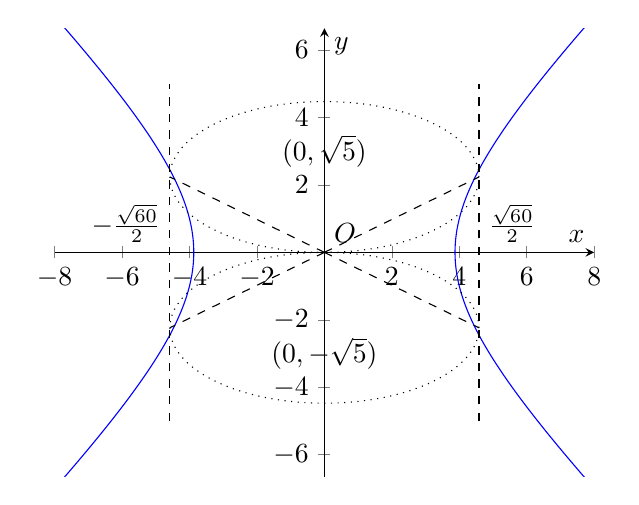
\begin{tikzpicture}
  \begin{axis}[xmin=-8,xmax=8,ymin=-5,ymax=5,axis equal,axis lines=middle,xlabel=$x$,ylabel=$y$]
    \addplot[blue,domain=-7.5:7.5,samples=200]({sqrt(15*(x^2/15+1))},{x});
    \addplot[blue,domain=-7.5:7.5,samples=200]({-sqrt(15*(x^2/15+1))},{x});
    \draw[dashed] (-4.5826,-5) -- (-4.5826,5);
    \draw[dashed] (4.5826,-5) -- (4.5826,5);
    \draw[dotted] (0,2.236) ellipse (4.5826 and 2.236);
    \draw[dotted] (0,-2.236) ellipse (4.5826 and 2.236);
    \node[above] at (0,2.236) {$(0, \sqrt{5})$};
    \node[below] at (0,-2.236) {$(0, -\sqrt{5})$};
    \node[above right] at (4.5826,0) {$\frac{\sqrt{60}}{2}$};
    \node[above left] at (-4.5826,0) {$-\frac{\sqrt{60}}{2}$};
    \node[above right] at (0,0) {$O$};
    \draw[dashed] (0,0) -- (4.5826,2.236);
    \draw[dashed] (0,0) -- (-4.5826,2.236);
    \draw[dashed] (0,0) -- (4.5826,-2.236);
    \draw[dashed] (0,0) -- (-4.5826,-2.236);
  \end{axis}
\end{tikzpicture}
\end{center}


\line(1,0){450}
\bigbreak \noindent 
\begin{large}
 \begin{center}
	 b) $\frac{(x-3)^2}{25}-\frac{(y-1)^2}{4}=1$
 \end{center} 
\end{large}
\bigbreak \noindent

\line(1,0){450}

\begin{center}
 Center: $(3,1)$ 
 \vspace{2mm}

$a = 5$
 \vspace{2mm}

$b = 2$
 \vspace{2mm}

$ c = \sqrt{29} $
\vspace{2mm}

Vertices: (8,1),(-2,1)
\vspace{2mm}

Foci: $(3 \pm\sqrt{29},1)$
\vspace{2mm}

slope = $\pm\frac{2}{5}$
Asymptotes: $y-1 =\pm \frac{2}{5}\left(x-3\right)$
\vspace{1mm}

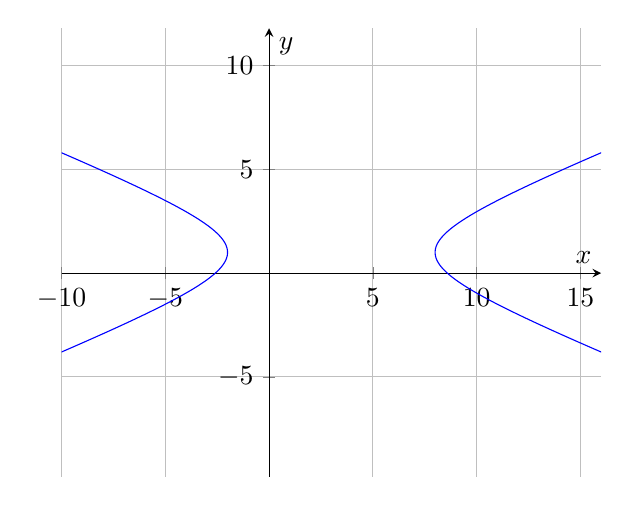
\begin{tikzpicture}
\begin{axis}[
    xmin=-10, xmax=16,
    ymin=-8, ymax=10,
    xlabel=$x$,
    ylabel=$y$,
    axis lines=center,
    axis equal,
    grid=both,
    restrict y to domain=-10:10 % limits the y-axis to prevent some unwanted lines
]
\addplot [blue, domain=-10:16, samples=200] ({3+5*cosh(x/5)}, {1+2*sinh(x/5)});
\addplot [blue, domain=-10:16, samples=200] ({3-5*cosh(x/5)}, {1+2*sinh(x/5)});
\end{axis}
\end{tikzpicture}
\end{center}
\bigbreak \noindent

\line(1,0){450}

\begin{center}
 \begin{large}
  c) $2 y^2-x^2+2 x+8 y+3=0$
 \end{large} 
\end{center}

\line(1,0){450}
\bigbreak
\begin{center}
   
\end{center}














\end{document}
